% uv-50m-alpha architecture (ultraviolet/model.py, preset "uv-50m-alpha"; 50.9M params incl. value embeddings).
% Build: pdflatex arch_uv_50m_alpha.tex
\documentclass[tikz,border=4pt]{standalone}
\usepackage{amsmath,amssymb}
\usetikzlibrary{positioning,fit,arrows.meta,calc,backgrounds}

\definecolor{cemb}{HTML}{FCE4D6}
\definecolor{cnorm}{HTML}{FFF2CC}
\definecolor{cattn}{HTML}{DDEBF7}
\definecolor{cglob}{HTML}{BDD7EE}
\definecolor{cmlp}{HTML}{E2EFDA}
\definecolor{cmisc}{HTML}{EDEDED}
\definecolor{cve}{HTML}{E4DFEC}

\tikzset{
  >={Stealth[length=2.2mm]},
  box/.style={draw, rounded corners=2pt, align=center, minimum height=6.5mm, minimum width=36mm,
              font=\small, inner sep=3pt},
  emb/.style={box, fill=cemb},
  nrm/.style={box, fill=cnorm, minimum height=5mm},
  att/.style={box, fill=cattn},
  mlp/.style={box, fill=cmlp},
  misc/.style={box, fill=cmisc},
  vebox/.style={box, fill=cve},
  small/.style={minimum width=17mm, font=\footnotesize},
  layer/.style={draw, rounded corners=1.5pt, minimum width=36mm, minimum height=5.2mm, font=\footnotesize,
                inner sep=1pt},
  op/.style={draw, circle, inner sep=0pt, minimum size=4.5mm, font=\footnotesize},
  note/.style={font=\scriptsize, align=left, text=black!70},
  line/.style={->, thick},
  title/.style={font=\bfseries},
}

\begin{document}
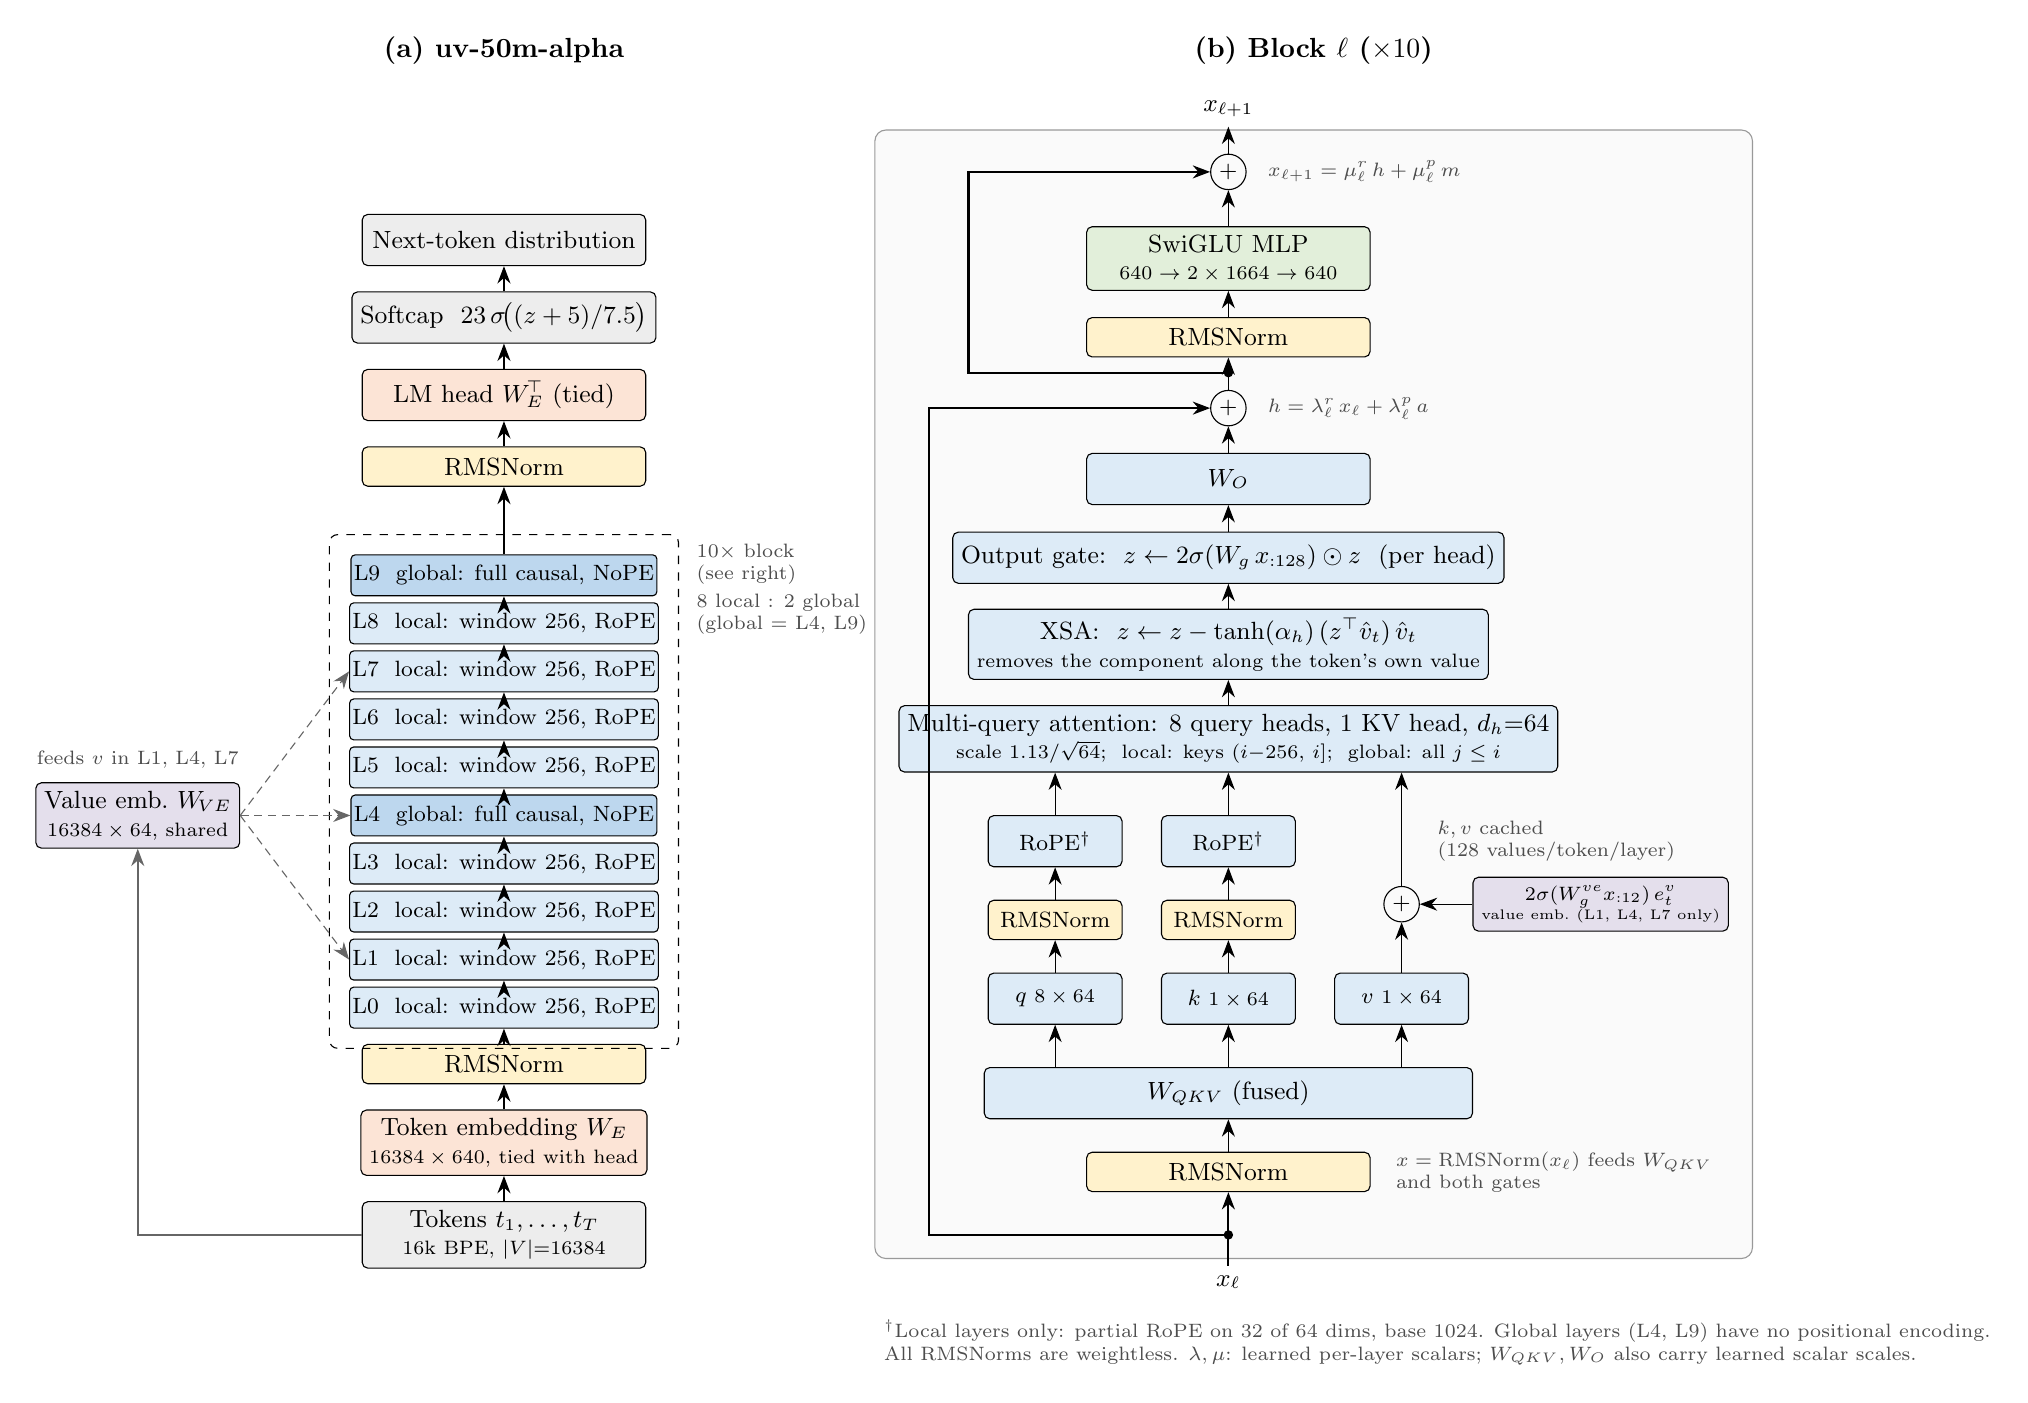
\begin{tikzpicture}[node distance=3.2mm and 6mm]

%% ======================= (a) model =======================
\node[misc] (tok) {Tokens $t_1,\dots,t_T$\\[-1pt]\scriptsize 16k BPE, $|V|{=}16384$};
\node[emb, above=of tok] (emb) {Token embedding $W_E$\\[-1pt]\scriptsize $16384\times640$, tied with head};
\node[nrm, above=of emb] (n0) {RMSNorm};

% layer stack, L0 at the bottom
\foreach \l in {0,...,9} {
  \pgfmathtruncatemacro{\g}{(mod(\l,5)==4) ? 1 : 0}
  \ifnum\g=1
    \node[layer, fill=cglob] (L\l) at ($(n0.north)+(0,4.6mm+\l*6.1mm)$)
      {L\l\ \ global: full causal, NoPE};
  \else
    \node[layer, fill=cattn] (L\l) at ($(n0.north)+(0,4.6mm+\l*6.1mm)$)
      {L\l\ \ local: window 256, RoPE};
  \fi
}
\draw[line] (n0) -- (L0);
\foreach \l [evaluate=\l as \n using int(\l+1)] in {0,...,8} { \draw[->] (L\l) -- (L\n); }
\node[draw, dashed, rounded corners=3pt, inner sep=2.5mm, fit=(L0)(L9)] (stack) {};
\node[note, anchor=north west] at ($(stack.north east)+(1mm,0)$)
  {$10\times$ block\\(see right)\\[2pt] 8 local : 2 global\\(global = L4, L9)};

% value embeddings
\node[vebox, minimum width=22mm, anchor=east] (ve) at ($(L4.west)+(-14mm,0)$)
  {Value emb.\ $W_{\!VE}$\\[-1pt]\scriptsize $16384\times64$, shared};
\draw[->, thick, black!60] (tok.west) -| ($(ve.south)$);
\foreach \l in {1,4,7} { \draw[->, densely dashed, black!60] (ve.east) -- (L\l.west); }
\node[note, above=0.5mm of ve, align=center] {feeds $v$ in L1, L4, L7};

\node[nrm, above=6mm of stack.north] (nf) {RMSNorm};
\draw[line] (L9) -- (nf);
\node[emb, above=of nf] (head) {LM head $W_E^{\!\top}$ (tied)};
\node[misc, above=of head] (cap) {Softcap\ \ $23\,\sigma\!\big((z+5)/7.5\big)$};
\node[misc, above=of cap] (out) {Next-token distribution};
\draw[line] (tok) -- (emb);
\draw[line] (emb) -- (n0);
\draw[line] (nf) -- (head);
\draw[line] (head) -- (cap);
\draw[line] (cap) -- (out);


%% ======================= (b) block =======================
\begin{scope}[xshift=92mm]
\node[font=\small] (xlab) at (0,-6mm) {$x_\ell$};
\coordinate (xin) at (0,0);
\node[nrm] (bn1) at (0,8mm) {RMSNorm};
\node[att, minimum width=62mm] (wqkv) at (0,18mm) {$W_{QKV}$ (fused)};

\node[att, small] (q) at (-22mm,30mm) {$q$\ \scriptsize $8\times64$};
\node[att, small] (k) at (0,30mm) {$k$\ \scriptsize $1\times64$};
\node[att, small] (v) at (22mm,30mm) {$v$\ \scriptsize $1\times64$};
\foreach \n in {q,k,v} { \draw[->] (wqkv.north -| \n) -- (\n); }

\node[nrm, small] (qn) at (-22mm,40mm) {RMSNorm};
\node[nrm, small] (kn) at (0,40mm) {RMSNorm};
\node[att, small] (qr) at (-22mm,50mm) {RoPE$^\dagger$};
\node[att, small] (kr) at (0,50mm) {RoPE$^\dagger$};
\draw[->] (q) -- (qn); \draw[->] (qn) -- (qr);
\draw[->] (k) -- (kn); \draw[->] (kn) -- (kr);

\node[op] (vadd) at (22mm,42mm) {$+$};
\draw[->] (v) -- (vadd);
\node[vebox, minimum width=25mm, font=\scriptsize, anchor=west] (veg) at (31mm,42mm)
  {$2\sigma(W_g^{ve} x_{:12})\, e^{v}_{t}$\\[-1pt]{\tiny value emb.\ (L1, L4, L7 only)}};
\draw[->] (veg) -- (vadd);

\node[att, minimum width=66mm] (sdpa) at (0,63mm)
  {Multi-query attention: 8 query heads, 1 KV head, $d_h{=}64$\\[-1pt]
   \scriptsize scale $1.13/\sqrt{64}$;\ \ local: keys $(i{-}256,\,i]$;\ \ global: all $j\le i$};
\draw[->] (qr) -- (qr |- sdpa.south);
\draw[->] (kr) -- (kr |- sdpa.south);
\draw[->] (vadd) -- (vadd |- sdpa.south);
\node[note, anchor=west] at ($(vadd.east |- kr)+(1mm,0)$) {$k,v$ cached\\(128 values/token/layer)};

\node[att, minimum width=66mm] (xsa) at (0,75mm)
  {XSA:\ \ $z \leftarrow z - \tanh(\alpha_h)\,(z^{\top}\hat v_t)\,\hat v_t$\\[-1pt]
   \scriptsize removes the component along the token's own value};
\node[att, minimum width=66mm] (ogate) at (0,86mm)
  {Output gate:\ \ $z \leftarrow 2\sigma(W_g\, x_{:128}) \odot z$\ \ (per head)};
\node[att] (wo) at (0,96mm) {$W_O$};
\draw[->] (sdpa) -- (xsa); \draw[->] (xsa) -- (ogate); \draw[->] (ogate) -- (wo);

\node[op] (add1) at (0,105mm) {$+$};
\draw[->] (wo) -- (add1);
\node[note, anchor=west] at ($(add1.east)+(1.5mm,0)$) {$h = \lambda^{r}_{\ell}\, x_\ell + \lambda^{p}_{\ell}\, a$};

\node[nrm] (bn2) at (0,114mm) {RMSNorm};
\node[mlp] (mlp) at (0,124mm) {SwiGLU MLP\\[-1pt]\scriptsize $640 \to 2\times1664 \to 640$};
\node[op] (add2) at (0,135mm) {$+$};
\node[note, anchor=west] at ($(add2.east)+(1.5mm,0)$) {$x_{\ell+1} = \mu^{r}_{\ell}\, h + \mu^{p}_{\ell}\, m$};
\node[font=\small] (xout) at (0,143mm) {$x_{\ell+1}$};
\draw[->] (add1) -- (bn2); \draw[->] (bn2) -- (mlp); \draw[->] (mlp) -- (add2); \draw[->] (add2) -- (xout);

% input and residual paths
\draw[thick] (xlab.north) -- (xin);
\draw[->, thick] (xin) -- (bn1);
\draw[->] (bn1) -- (wqkv);
\draw[->, thick] (xin) -- (-38mm,0) |- (add1.west);
\coordinate (hs) at (0,109.5mm);
\draw[->, thick] (hs) -- (-33mm,109.5mm) |- (add2.west);
\fill (xin) circle (0.6mm); \fill (hs) circle (0.6mm);
\coordinate (rcorner) at (-38mm,0);
\node[note, anchor=west] at ($(bn1.east)+(2mm,0)$) {$x=\mathrm{RMSNorm}(x_\ell)$ feeds $W_{QKV}$\\and both gates};

\begin{scope}[on background layer]
  \node[draw=black!40, rounded corners=4pt, fill=black!2, inner sep=3mm,
        fit=(bn1)(wqkv)(veg)(sdpa)(xsa)(ogate)(add2)(rcorner)] (blk) {};
\end{scope}
\node[title, anchor=south] (tb) at ($(blk.north)+(0,7mm)$) {(b) Block $\ell$ ($\times 10$)};
\node[note, anchor=north west] at ($(blk.south west)+(0,-6.5mm)$)
  {$^\dagger$Local layers only: partial RoPE on 32 of 64 dims, base 1024. Global layers (L4, L9) have no positional encoding.\\
   All RMSNorms are weightless. $\lambda,\mu$: learned per-layer scalars; $W_{QKV}, W_O$ also carry learned scalar scales.};
\end{scope}
\node[title] at (out |- tb) {(a) uv-50m-alpha};

\end{tikzpicture}
\end{document}
